\section{Treatment Plan (TP) Optimization (BOO)}
\begin{frame}
\frametitle{Treatment Plan (TP) Optimization}
\centering Left blank intentionally.
\end{frame}

\begin{frame}
\frametitle{IMRT TP Overview}
\begin{itemize}
	\item IMRT delivers geometrically-shaped, high-precision photons to tumors in a beam orientation optimization (BOO) process. %by modulating the intensity of the radiation beam from a robot's eye-view
	%
	%\item Treatment planning  involves organs contouring in a target volume
	%
	%\item Each (photon) beam to be delivered is comprised of beamlets, typically aimed from the same angle
	%
	\vspace{0.3cm}
	%
	\item The \textbf{BOO problem} aims to find the right beam angle combinations from which to deliver radiation intensities.
	%
	\vspace{0.2cm}
	%
	\begin{itemize}
		\item essentially a combinatorial optimization problem 
		\vspace{0.2cm}
		%
		\item traditional methods fail at \underline{real-time feasible results\footnote{Current approaches take too long, and are often not optimal.}}.
	\end{itemize}
	\vspace{0.1cm}
	%
	\item Afterwards, the intensity of the fluence is modulated in a \textbf{fluence map optimization} (FMO) process.
%
\end{itemize}
\end{frame}

\begin{frame}
	\frametitle{IMRT Treatment Plan Flowchart}
	\centering
	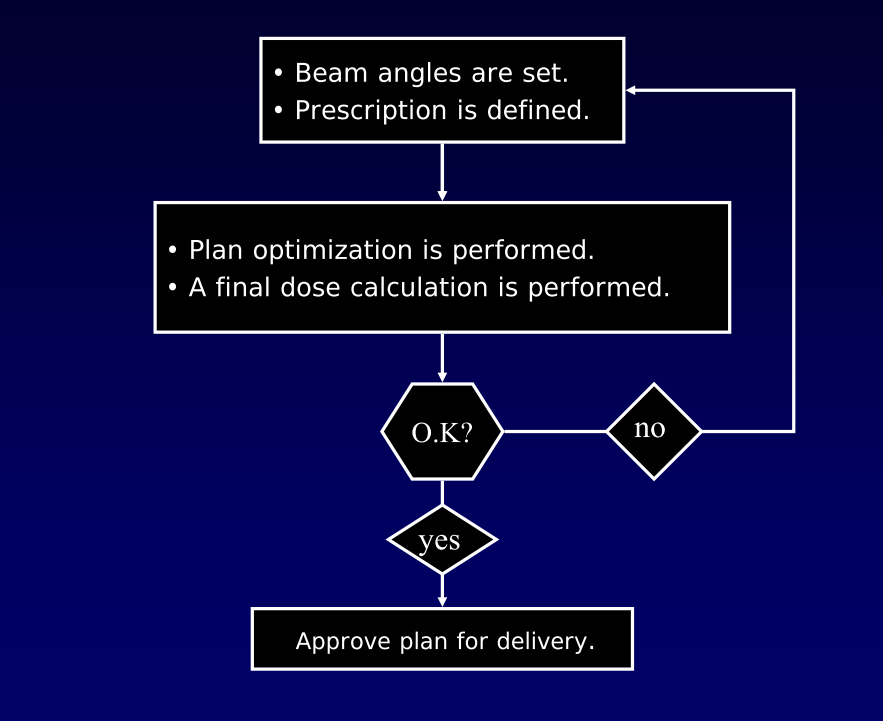
\includegraphics[width=.75\columnwidth]{figures/flowchart.png} \\
	\tiny Reprinted from ``IMRT Optimization Algorithms. David Shepard. Swedish Cancer Institute. AAPM 2007."
\end{frame}

\begin{frame}
\frametitle{Problem Setup}
\begin{columns}[c]
	\begin{column}{0.45\textwidth}
		\begin{itemize}
			\item Given biological statement of prescriptions %is expressed in a numerical objective function
			%
			\begin{itemize}
				\item find a numerical \textbf{objective function}
				%
				\item accompanied by \textbf{constraints}
			\end{itemize}
			%
			\item \textbf{Challenge}
			%
			\begin{itemize}
				\item a scalar-valued objective function usually not sufficient %
			\end{itemize}
		\end{itemize}
	\end{column}
	%
	\begin{column}{0.45\textwidth}
		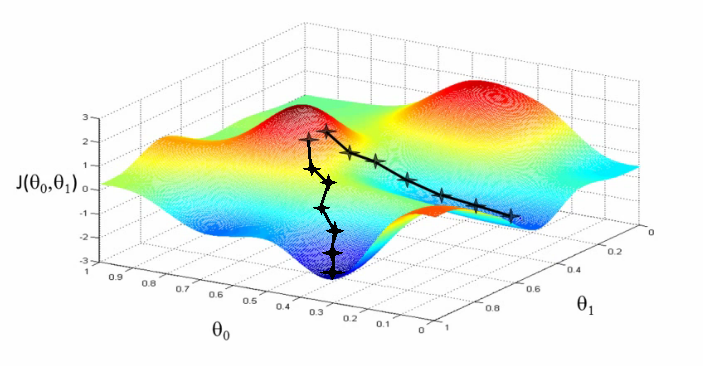
\includegraphics[width=\linewidth, height=.70\linewidth]{figures/nonconvex.png}
		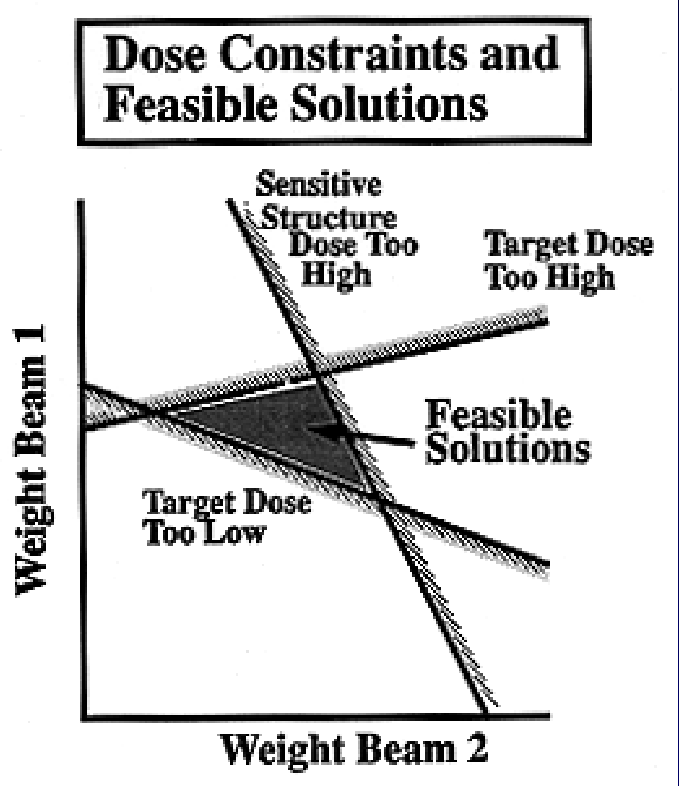
\includegraphics[width=\linewidth, height=.70\linewidth]{figures/dose_constraints.png}
		\\ \tiny \centering Courtesy of David Shepard
	\end{column}
	%
\end{columns}
\end{frame}

\begin{frame}
\frametitle{Dosimetric Constraints}
\begin{itemize}
	\item Constraints $\neq$ \textbf{optimal solution} 
	%
	\item  Constraints define what constitutes an \textbf{acceptable solution}
	%
	\item With \textbf{conflicting constraints} (almost always), feasible solution is near impossible
	%
	\begin{itemize}
		\item OARs must have minimum dose
		%
		\item Planning Target Volumes (PTVs) must receive maximum dose
		%
		\item OARs and Tumors may be juxtaposed/intersect 
		%
		\item DVH constraints 
		%
		\begin{itemize}
			\item \eg specified as  60\% of left femoral head may not exceed a dose of 40 Gy	
		\end{itemize}%, \textit{}	
	\end{itemize}
	
\end{itemize}
\end{frame}

\begin{frame}
\frametitle{Common Problem Formulation}
\begin{itemize}
	\item Maximize weighted least square dose from for PTVs
	%
	\item Minimize weighted least square dose for OARs
	%
	\item DVH-based goal treatments
\end{itemize}
	\hrulefill
	%
	\begin{itemize}
		\item Current Approaches and Limitations
		%
		\begin{itemize}
			\item Stochastic optimization approaches: simulated annealing; genetic algorithms and gradient search, or a combination of genetic and gradient search algorithms
			%
			\item Mixed-integer programming, branch and cut/bound algorithms, beam angle elimination algorithms
		\end{itemize}
	\item General weakness: Feasible solution takes too long to find.
	\end{itemize}
\end{frame}

\begin{frame}
\frametitle{Our approach}
\begin{itemize}
	%
	\item Automate the \textbf{beam search} problem
	%
	\vspace{0.3cm}
	%
	\item \textbf{Ultimate goal} is real-time beam angle prediction given a target volume 
	%
	\vspace{0.3cm}
	%
%	\item And the intensity modulation process	
%	%
%	\vspace{0.3cm}
	%
	\item Drawing ideas from 
	%
	\vspace{0.3cm}
	%
	\begin{itemize}
		\item \textbf{pattern recognition};
		%
		\vspace{0.3cm}
		%
		\item \textbf{monte carlo evaluations};
		%
		\vspace{0.3cm}
		%
		\item \textbf{game simulations}; and
		%
		\vspace{0.3cm}
		%		
		\item \textbf{approximate dynamic programming}
	\end{itemize}
\end{itemize}
\end{frame}

\begin{frame}
\frametitle{What we do}
\begin{itemize}
	\item Formulate BOO problem into a large game planning strategy
	%
	\vspace{0.3cm}
	%
	\item Neural fictitious self-play~[\cite{Heinrich}], to refine policy predictions
	%
	\begin{itemize}
		\item \textbf{purpose}: drive policy weights to a \textbf{saddle equilibrium}
		%
	\end{itemize}
	%
	\vspace{0.3cm}
	%
	\item a deep neural network models the nonlinear dynamical system (patient's geometry, robot-linac setup)
	%
	\vspace{0.3cm}
	%
	\begin{itemize}
		\item generating a policy that guides MCTS simulations for two  players in a zero-sum Markov game
	\end{itemize}
	%
\end{itemize}
\end{frame}

\begin{frame}
	\frametitle{What we do}
	\begin{itemize}
		\item In each episodic markov decision process (MDP) setting, an MCTS lookout strategy guides transition from one beam angle set to another 
		%
		\vspace{0.3cm}
		%
		\item Each player in a two-player Markov game  finds a best response strategy to their opponent's average strategy 
		%
		\vspace{0.3cm}
		%
		\begin{itemize}
			\item driving the policy weights  toward an approximate \textbf{saddle equilibrium} ~\cite{Heinrich}.
		\end{itemize}
	\end{itemize}
\end{frame}

\begin{frame}
	\frametitle{Problem Setup}
	\begin{itemize}
		\item Let state of the dynamical system be $\netstate \in \mc{S}$
		%
		\vspace{0.3cm}
		%
		\item To be controlled by a discrete action $\action \in \actionspace$
		%
		\vspace{0.3cm}
		%
		\item States evolve according to an (unknown) dynamics $p(\netstate_{t+1}|\netstate_t, \action_t)$ (to be learned)
		%
		\vspace{0.3cm}
		%
		\item Beam angle combination search task defined by a reward function, $R_t = \sum_{t=1}^{N}\gamma^{t-1} \reward(\netstate_t, \action_t)$
		%
		\vspace{0.3cm}
		%
		\begin{itemize}
			\item Can be found by recovering a policy, $p(\action_t | \netstate_t; \psi)$
			%
		\end{itemize}
		%
		\vspace{0.3cm}
		%
		\item From now on, we will write $p(\action_t | \netstate_t; \psi)$ as $\policy_\psi(\action_t|\netstate_t)$.
	\end{itemize}
\end{frame}

\frame{
\frametitle{Preliminaries}
\begin{itemize}
	\item Suppose the first player is $p_1$, and the second player is $p_2$
	%
	\item $p_1$ chooses its action under a (stochastic) strategy, $\pi^{p_1} = \{\pi^{p_1}_0, \pi^{p_1}_1, \ldots, \pi^{p_1}_{T}\} \subseteq \Pi^{p_1}$
	%
	\begin{itemize}
		\item minimizing the game's outcome $\zeta$
	\end{itemize}
	%
	\item $p_2$'s actions are governed by a policy $\pi^{p_2} =\{ \pi^{p_2}_0, \pi^{p_2}_1, \ldots , \pi^{p_2}_{T}\} \subseteq \Pi^{p_2}$
	%
	\begin{itemize}
		\item $p_2$ seeks to maximize $\zeta$ in order to guarantee an equilibrium solution for a game without saddle point.
	\end{itemize}
	%
	\item $\Pi^{p_i}$ is the set of all possible nonstationary markovian policies
\end{itemize}
}

\begin{frame}
	\frametitle{Preliminaries}
	\begin{itemize}
		\item Each player bases its decision on a random event's outcome 
		%
		\begin{itemize}
			\item  generating a \textbf{mixed strategy} determined by \textbf{averaging the outcome} of individual plays.
		\end{itemize}
	%
	\item Both players constitute a two-player \textbf{stochastic action selection strategy}, $\policy(\netstate, \action) = Pr(\action | \netstate):=\{\policy^{p_1}, \policy^{p_2}\}$ that gives the probability of selecting moves in any given state
	%
	\item Suppose the game simulation starts from an initial condition $\netstate_0$.
	%
	\end{itemize}
	%
\end{frame}

\begin{frame}
\frametitle{Preliminaries}
%
\begin{itemize}
	\item One may write the optimal \textbf{reward-to-go} value function for state $s$ in stage $t$, with horizon length $T$ as 
	%
	\begin{align}
	V_t^*(\netstate) & = \inf_{\pi^{p_1} \in \Pi^{p_1}} \sup_{\pi^{p_2} \in \Pi^{p_2}} \bb{E}\left[\sum_{i=t}^{T-1} V_t(\netstate_0, f(\netstate_t, \pi^{p_1}, \pi^{p_2})) \right], \nonumber \\
	&	\qquad  \netstate \in S, \, t = 0, \ldots, H-1 \nonumber
	\end{align}
	%
	\item where the terminal value $V_T^*(\netstate) = 0, \, \, \forall \, s \in S$;
	%
	\item $f(\cdot)$ represents the unknown system dynamics
	%
	\item $\pi^{p_1}$ and $\pi^{p_2}$ contain the action/control sequences $\{\action^{p_1}_t\}_{0 \le t \le T}$ and $\{\action^{p_2}_t\}_{0 \le t \le T}$
	%
\end{itemize} 
%
\end{frame}

\begin{frame}
	\frametitle{Preliminaries}
	%
	\begin{itemize}
		\item The \textbf{saddle point strategies} for an optimal control sequence pair $\{\action^{p^*_1}_t, \action^{p^*_2}_t\}$  can be recursively obtained by optimizing a state-action value cost, $\cost_t(\netstate, \action)$ 
		%
			\begin{align}
		V_t^*(\netstate) = V_t^*(\netstate_t, \pi^{p_1}_t, \pi^{p_2}_t) &= \min_{\pi^{p_1} \in \Pi^{p_1}} \max_{\pi^{p_2} \in \Pi^{p_2}} V^\star_t(\netstate_t, \pi^{p_1}, \pi^{p_2})  \nonumber \\
		%
		& \quad \forall \netstate_t \in \mc{S}, \pi^{p_1} \in \Pi^{p_1}, \pi^{p_2} \in \Pi^{p_2}.
		\label{eq:minimax} \nonumber
		\end{align}
	\end{itemize}
	%
	such that
	\[
	V^\star_{p_1} \le V^\star \le V^\star_{p_2} \quad \forall \,  \{\pi^{p_1}_t, \pi^{p_2}_t\}_{0 \le t\le T}.
	\]
	where $V^\star_{p_i}$ are the respective optimal values for each player. 
\end{frame}

\begin{frame}
%
	\frametitle{Preliminaries}
	%
	\begin{itemize}
%		\item 
%		$Q(\netstate, \action)$  can be recovered from the reward function $R(\netstate, \action)$ and transition function, $P(\netstate, \action)$ as
%		\[
%		\cost_t^*(\netstate_t, \pi^{p_1}_t, \pi^{p_2}_t) = R(\netstate, \action) + \gamma \sum_{x \in S}^{}P(\netstate, \action)(x) V^\star_{t+1}(x).
%		\]
		%
		%\item The action pair can be readily recovered with dynamic programming -- transforming the optimization over the entire policy  to a step-wise `min-max' over each control sequence $\{\action^{p_1}_t, \action^{p_2}_t\}_{0 \le t \le T}$. 
		%
		\item Under ideal conditions, we'd like to find the optimal value function under perfect play
		%
		\item \textbf{Caveat:} BOO exhibits Bellman's curse of dimensionality.
		%
		\item What to do?
		\begin{itemize}
			\item derive an \textbf{approximately optimal} value $V_\psi^\star(\netstate)$
			%
			\item by continually estimating the value function $v^p_\psi(\netstate)$ using \eg a policy parameterized by a large function approximator
		\end{itemize}  
	\end{itemize}
\end{frame}

\begin{frame}
	\frametitle{Beam Angles Representation}
	%\begin{figure}[tb!]%
		\centering
		\includegraphics[width=0.23\columnwidth]{../../BOO/figures/beams/beam_010.jpg}
		%
		\includegraphics[width=0.23\columnwidth]{../../BOO/figures/beams/beam_082.jpg} 
		%
		\includegraphics[width=0.24\columnwidth]{../../BOO/figures/beams/beam_166.jpg} \\
		%
		\centering
		[Left to right]: Beam $10^\circ$, Beam $82^\circ$, Beam $166^\circ$ \\
		%
		\includegraphics[width=0.23\columnwidth]{../../BOO/figures/beams/beam_210.jpg}
		%
		\includegraphics[width=0.23\columnwidth]{../../BOO/figures/beams/beam_286.jpg}
		%
		\includegraphics[width=0.24\columnwidth]{../../BOO/figures/beams/beam_342.jpg}
		\\
		\centering
		[Left to right]: Beam $210^\circ$, Beam $286^\circ$, Beam $342^\circ$ \\
\end{frame}

\frame{
\frametitle{State Representation}
	\includegraphics[width=.63\columnwidth,height=0.38\columnwidth]{../../BOO/figures/new_architecture_no_ellipsis.png}
%
\includegraphics[width=.35\columnwidth,height=0.3\columnwidth]{../../BOO/figures/beams/beam_block.png}
\footnotesize [Left]: Concatenation of the target volume masks and the beam angles before feeding the input planes to the residual tower neural network. The first six planes (top-most mask of left figure) contain the delineated organs and the PTV. This is concatenated with a block of $m$ beams from the current time step, regressed to the previous 5 time steps (here, $5$ was heuristically chosen). [Right]: Each beam angle in a beam block is  represented as shown. Together with the target volume, these form an input plane of size $36 \times \slice \times W \times H$ to the policy/value neural network tower of residual blocks.
}

\begin{frame}
	\frametitle{Methods}
	\begin{itemize}
		\item A head of this network approximates the value function, $v(\netstate_\tidx)$, for the current state, and the feedback policy $\pi(\netstate_\tidx)$
		%
		\item A second head serves as an ad-hoc deep Q action-value network [see~\cite{atarigames}] 
		\begin{itemize}
			\item producing Q-values over the possible action spaces for the partially observable markov decision process (POMDP).
		\end{itemize}
	\item We run Monte Carlo simulations with the search probabilities, $\pi_t = \alpha_{\psi_{i-1}}(\netstate_\tidx)$, generated from a previous iteration of training the neural network $p, v = f_{\psi_{i-1}}(\netstate)$.
	\end{itemize}
\end{frame}

\begin{frame}
	\frametitle{Methods: Search}
	\begin{itemize}
		\item Formulated as a bandit search that imposes a regret term on the $\qfunc$-value
		%
		\item During the planning process, we estimate a \textit{value}, $v(\state_t)$, that estimates the optimality of a beam block; 
		%
		\item In parallel, we refine the deep neural network policy by optimizing its weight in a separate thread. 
		%
		\begin{itemize}
			\item This player's weights are continually written to a shared memory such that its values are available to the MCTS search thread. 
			%
			\item Network parameters updated  by a \textbf{mixed strategy} which combines its \textbf{pure strategy}, which is a best response to the \textbf{average pure strategy} of a fictitious opponent.
		\end{itemize}
	\end{itemize}
\end{frame}

\begin{frame}
\frametitle{Methods: Search}
\begin{itemize}
	\item $\qfunc$-value defined as 	
	%
	\begin{align}
	\bar{Q}(\netstate, \action) &= \qfunc_j(\netstate, \action) + c  \sqrt{\dfrac{2 \text{ ln} \,\, n(s)}{N(s,a}}, \\
	a^\star &= \arg \max_\action \bar{Q}(\netstate, \action)
	\label{eq:upper_conf}
	\end{align}
	%
	\hrulefill \\
	Fluence Map Optimization
	\begin{itemize}
		\item Suppose $\voxtot$ is the total discretized of voxels of interest ($VOI$'s) in a target volume
		%
		\item Suppose $\beamlets_1 \cup \beamlets_2 \cup \ldots \cup \beamlets_n \subseteq \beamlets$ represents the partition subset of a  beam $\beamlets$, 
		\begin{itemize}
			\item where $n$ is the total number of beams from which radiation can be delivered
		\end{itemize}
	\end{itemize}
\end{itemize}
\end{frame}

\begin{frame}
\frametitle{Methods: Fluence Map Optimization}
\begin{itemize}
	\item Suppose further that $\dij(\beamangle_k)$ is the matrix that describes each dose influence, $d_i$.
	%
	\begin{itemize}
		\item  delivered to a discretized voxel, $i$, in a volume of interest, $VOI_h \, (h = 1, \ldots, \voxtot)$, from a beam angle, $\beamangle_k$, $k \in \{1, \ldots, n\}$
	\end{itemize}
	%
	\item We compute the matrix $\dij(\beamangle_k)$ by calculating each $d_i$ for every bixel, $j$, at every $\varphi^\circ$, resolution, where $j \in \beamlets_k$
	%
	\begin{itemize}
		\item ending up with an ill-conditioned (\textit{sparse}) matrix, $\dij(\beamangle_k)$, which consists of the dose to every voxel, $i$, incident from a beam angle, $\beamangle_k$ at every $360^\circ/\varphi^\circ$
		%
	\end{itemize}
\end{itemize}
\end{frame}

\begin{frame}
	\frametitle{Methods: FMO problem definition}
	\begin{itemize}
		\item The fluence problem is to find the values of decision variables, $\bixel_j$, for which $d_i$ to the tumor is maximized, while simultaneously minimizing the $d_i$ to critical structures
		%
		\item For the voxels in a target volume, 
		
		\begin{itemize}
			\item let a weighted quadratic objective minimize the $l_2$ distance between a pre-calculated dose $\Amat \primal$, and a doctor's prescribed dose, $\textbf{b}$
			%
			\item let a weighted quadratic objective maximizes the $l_2$ distance between $\Amat \primal$ (where $\primal$ represents the vectorized bixels, $\bixel_j$) and $\textbf{b}$
		\end{itemize}
	\end{itemize}
\end{frame}

\begin{frame}
\frametitle{Methods: FMO problem definition}
\begin{itemize}
	\item The pre-calculated dose term is given by $\Amat\primal = \{\sum_s\frac{w_s}{v_s} \dij^s \primal_s  \, | \, \dij \in \bb{R}^{n \times l}, n>l\}$%, which is a combination of the dose components that belong to OARs and those that belong to PTVs. 
	
	\vspace{0.2cm}
	%
	\item Let $w_s = \{\underline{w}_s, \bar{w}_s\}$ be the respective underdosing and overdosing weights for the OARs and PTVs, and $v_s$ represents the total number of voxels in each structure.
	%
	\vspace{0.2cm}
	\item We propose the following cost
	%
	\small \begin{align}
	\frac{1}{v_s}\sum_{s \in \text{OARs}}  \|(b_s - \underline{w}_s \dij^s \primal_s)_+ \|_2^2 + \frac{1}{v_s}\sum_{s \in \text{PTVs}}  \|(\bar{w}_s \dij^s \primal_s - b_s)_+\|_2^2 
	\label{eq:fmo_cost}
	\end{align}
	%
\end{itemize}
\end{frame}

\begin{frame}
\frametitle{Methods: FMO}
	\begin{itemize}
		\item Rewriting the objective, subject to nonnegative bixel intensity constraints, we have the minimization problem
		\[
		\min \frac{1}{2}\|A \textbf{x} - \textbf{b}\|_2^2  \quad \text{ subject to }  x \ge 0.
		\]
		%
		\item The Lagrangian becomes
		%
		\[
		L(\primal, \bm{\lambda}) = \min \frac{1}{2}\|A \textbf{x} - \textbf{b}\|_2^2 - \bm{\lambda}^T \primal.
		\]
		\item Since we are solving a large scale problem, we use the ADMM algorithm
		%
		\item Introducing an auxiliary variable $\textbf{z}$, we have 
		\begin{align}
		\min_{\primal} \frac{1}{2}\|\Amat \primal - \textbf{b}\|_2^2,
		\,\,\, \text{ subject to }  \admmvar = \primal, \,\, \admmvar \ge 0, \nonumber
		\end{align}
	\end{itemize}
\end{frame}


\begin{frame}
\frametitle{Methods: FMO}
\begin{itemize}
	\item Solving either the $\primal$ and $\admmvar$ sub-problems, we have
	%
	\begin{align}
	\primal^{k+1} = \left(\Amat^T\Amat + \rho \bm{I}\right)^{-1}\left(\Amat^T\bm{b}+ \rho \admmvar^k - \bm{\lambda}^k\right).
	\label{eq:admm_xupdate}
	\end{align}
	%
	\item And using the soft-thresholding operator, $S_{\bm{\lambda}/\rho}$, we find that
	\begin{align}
	\admmvar^{k+1} = S_{\bm{\lambda}/\rho}\left(\primal^{k+1} + \bm{\lambda}^k \right),
	\end{align}
	%
	where $S_{\bm{\lambda}/\rho}(\tau) = (x - \bm{\lambda}/\rho)_+ - (-\tau - \bm{\lambda}/\rho)_+$.  $\bm{\lambda}$ is updated as
	\begin{align}
	\bm{\lambda}^{k+1} = \bm{\lambda}^k - \gamma (\admmvar^{k+1} - \primal^{k+1}),
	\end{align}
	where $\gamma$ is a parameter that controls the step length.
\end{itemize}
\end{frame}


\subsection{Game Tree Simulation}
\begin{frame}
	\frametitle{Game Tree Simulation}
	%
	\begin{itemize}
		\item For $b^d$ possible move sequences for a robot-patient setup 
		\begin{itemize}
			\item $b = $ beam angles chosen to construct a fluence 
			%
			\item $d = $ is the total number of discretized angles.
		\end{itemize}
	%
	\item  Suppose $b=180$ and $d = 5$, we have $180^{5}$ possible search directions
	%
	\item Exhaustive search becomes real-time infeasible.
	\end{itemize}%We  leverage Monte Carlo simulations, encouraged by their recent success in large games  \cite{Chung2005monte, Silver2016, Silver2017}, to break the curse of dimensionality~\cite{Bellman1957}.
\end{frame}

\begin{frame}
\frametitle{Game Tree Simulation; Approach}
%
\begin{itemize}
	\item Simulate a game of \textbf{perfect recall} 
	%
	\begin{itemize}
		\item a sequential simulation of different beam angle combinations g
		%
		\item guided by probabilities obtained from a two-player zero-sum game of neural FSP 
	\end{itemize}
	%
	\item  the probability distribution is over the possible beam angle subsets, $\beamangle^j$, in the beam angle space, , $\beamsall$
	%
	\item This strongly discourages classical beam s approaches
\end{itemize}%We  leverage Monte Carlo simulations, encouraged by their recent success in large games  \cite{Chung2005monte, Silver2016, Silver2017}, to break the curse of dimensionality~\cite{Bellman1957}.
\end{frame}

\begin{frame}
	\frametitle{Game Tree Simulation}
	\begin{itemize}
		\item Network roll-out policy then efficiently guides the tree's game, $\Gamma$ toward a \textit{best-first} set of  beam angle candidates
		%
		\item Best-first leaf node encountered is the child node with the highest reward in the tree
		%
		\item Essentially, a sampling-based lookout algorithm 
		
		\begin{itemize}
			\item Focuses learning on regions of the state space that are likely to have a good fluence
		\end{itemize}  
	\end{itemize}
\end{frame}


\frame{
	\frametitle{MCTS Simulation}
	\begin{itemize}
		\item After each simulation iteration, a `best move' for the current beam block is selected, as computed by the tree search
		
		\item 
		Four steps are applied at each iteration of the simulation for each player in $\{p_1, p_2\}$, viz,
		
		\begin{itemize}
			\item \textit{Selection}: starting at a root node, we recursively apply a child selection policy to navigate the branches of the tree until an expandable node is encountered. %A node is defined to be expandable as defined in \autoref{def:expandable}.
			\item \textit{Expansion}: we iteratively add one or more children to the current node, based on the available move probabilities%, \eqref{eq:upper_conf}%, $\netprobs$
		\end{itemize}
	\end{itemize}
}

\frame{
\frametitle{MCTS}
\begin{itemize}
	\item MCTS Steps (cont'd)
	\begin{itemize}		
		\item \textit{Simulation}: a simulation from the beam angles in the new node is carried out to determine the optimal fluence objective function
		\item \textit{Back-up}: from the \textit{leaf node} (encountered during the expansion procedure), the lookout simulation is ``backed up" through its direct nodal ancestors -- updating each node's statistics as we traverse the current node up to the root node.
	\end{itemize}
\end{itemize}
}
\begin{frame}
	\frametitle{Deep BOO MCTS Algorithm}
	\centering
	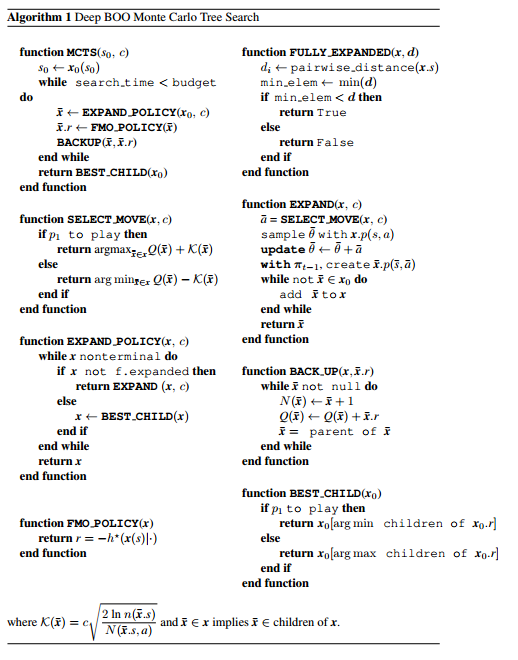
\includegraphics[width=0.5\columnwidth]{figures/mcts_alg.png}
\end{frame}

\begin{frame}
\frametitle{Transition Slide}
\centering This page is left blank intentionally.
\end{frame}
